\chapterheading{5}{PHƯƠNG ÁN CÀI ĐẶT VÀ BỘ TÍNH THAM CHIẾU}
\setcounter{section}{5}
\setcounter{subsection}{0}
\setcounter{subsubsection}{0}

\subsection{Phạm vi cài đặt và công nghệ lựa chọn}
Chương này trình bày phương án tổ chức cài đặt từ kiến trúc ở Chương 4. Cấu trúc thư mục, cấu hình và mã giả là đặc tả triển khai. Phần đã được thực thi trong báo cáo là bộ tính khoảng thời gian tham chiếu và các chương trình đánh giá đi kèm. Các mô-đun camera, máy trạng thái, API và giao diện còn được trình bày ở mức phương án tích hợp.

Phương án cài đặt kế thừa nền tảng Python/FastAPI của mã nguồn ban đầu và tổ chức lại miền nghiệp vụ theo nhân viên, camera và khoảng hiện diện. Python được dùng cho ứng dụng camera, thị giác máy tính, máy chủ ứng dụng và tiến trình xử lý nền báo cáo. OpenCV xử lý khung hình và thao tác hình học, Ultralytics YOLOv8 cung cấp bộ phát hiện, ByteTrack được tích hợp qua bộ theo dõi của Ultralytics hoặc lớp tích hợp riêng, facenet-pytorch cung cấp MTCNN và InceptionResnetV1 cho vector đặc trưng khuôn mặt. FastAPI cung cấp REST/WebSocket \cite{fastapi}, SQLAlchemy 2.0 ánh xạ dữ liệu \cite{sqlalchemy}, PostgreSQL lưu dữ liệu quan hệ \cite{postgresql} và Redis hỗ trợ trạng thái tạm cùng kênh phân phối thông báo khi triển khai nhiều tiến trình \cite{redis}. Redis Pub/Sub không bảo đảm phát lại thông điệp đã mất, do đó sự kiện nghiệp vụ cần được lưu bền vững và xác nhận riêng.

Phương án triển khai sử dụng Docker Compose ở phía máy chủ. Ứng dụng camera có thể chạy độc lập trên thiết bị biên có GPU hoặc CPU phù hợp. Việc tách ứng dụng phía máy khách/máy chủ cho phép đặt video gần nguồn camera và chỉ truyền dữ liệu dẫn xuất.

\begin{table}[H]
\centering
\caption{Các công nghệ chính}
\label{tab:tech-stack}
\begin{tabularx}{\textwidth}{p{3.4cm}p{4.2cm}X}
\toprule
\textbf{Thành phần} & \textbf{Công nghệ} & \textbf{Vai trò}\\
\midrule
Thị giác máy tính & Python, OpenCV, Ultralytics & Khung hình, quan sát phát hiện, hình học\\
Bộ phát hiện & YOLOv8n & Người và điện thoại\\
Bộ theo dõi & ByteTrack & Theo dõi đa đối tượng\\
Danh tính & facenet-pytorch & cắt vùng mặt bằng MTCNN + vector đặc trưng FaceNet\\
Máy chủ ứng dụng & FastAPI & REST, WebSocket, xác thực\\
ORM/DB & SQLAlchemy, PostgreSQL & Dữ liệu quan hệ/trạng thái hiện tại\\
Cache/hàng đợi & Redis & Phân phối cập nhật, tác vụ/trạng thái hỗ trợ\\
Sinh báo cáo & Jinja2/HTML/PDF & Báo cáo ngày/nhân viên\\
Triển khai & Docker Compose & Máy chủ ứng dụng, DB, Redis\\
\bottomrule
\end{tabularx}
\end{table}

\subsection{Cấu trúc kho mã nguồn đề xuất}
Các gói chức năng được tổ chức theo miền nghiệp vụ nhân viên, camera, hiện diện và thời gian. Cấu trúc thư mục đề xuất như sau:
\begin{Verbatim}[fontsize=\small,breaklines=true,breakanywhere=true]
project/
|-- main.py
|-- config/
|   |-- vision.yaml
|   `-- policies.yaml
|-- src/
|   |-- perception/
|   |   |-- pipeline.py
|   |   |-- yolo_detector.py
|   |   |-- face_embedder.py
|   |   `-- perception_result.py
|   |-- tracking/
|   |   |-- person_tracker.py
|   |   |-- tracked_person.py
|   |   `-- identity_associator.py
|   |-- workplace/
|   |   |-- work_area.py
|   |   |-- roi_manager.py
|   |   `-- geometry.py
|   |-- presence/
|   |   |-- presence_state.py
|   |   |-- presence_tracker.py
|   |   `-- work_time_aggregator.py
|   |-- phone_usage/
|   |   |-- phone_associator.py
|   |   |-- phone_usage_state.py
|   |   `-- phone_usage_tracker.py
|   |-- client/backend_client.py
|   `-- reporting/
|-- backend/
|   |-- models.py
|   |-- auth.py, authorization.py
|   |-- ws_schemas.py, ws_manager.py
|   |-- routers/
|   `-- templates/, static/
|-- tests/, backend/tests/
`-- docker-compose.yml
\end{Verbatim}

Cấu trúc đề xuất cho phép tái sử dụng các thành phần xác thực, phân quyền, quản lý WebSocket, sinh báo cáo và đóng gói Docker. Các chức năng không thuộc bài toán hiện diện được đặt ngoài phạm vi triển khai.

\subsection{Cấu hình tập trung}
Tệp \texttt{vision.yaml} lưu tham số camera, bộ phát hiện, bộ theo dõi, ROI, danh tính và máy trạng thái. Ví dụ:
\begin{Verbatim}[fontsize=\small,breaklines=true,breakanywhere=true]
camera:
  source: rtsp://...
  inference_size: 640
  telemetry_interval_sec: 1.0

detector:
  model: yolov8n.pt
  person_conf: 0.10
  phone_conf: 0.50
  iou: 0.60

tracker:
  type: bytetrack
  track_high_thresh: 0.50
  track_low_thresh: 0.10
  track_buffer: 30

presence:
  enter_sec: 2.0
  gap_sec: 5.0
  min_valid_ratio: 0.70

phone_usage:
  enter_sec: 3.0
  exit_grace_sec: 2.0
  association_threshold: 0.60
\end{Verbatim}
Ngưỡng lọc người ở đầu ra bộ phát hiện không được lớn hơn ngưỡng liên kết thấp của ByteTrack, nếu không các hộp có độ tin cậy thấp sẽ bị loại trước bước ghép thứ hai. Các giá trị trong ví dụ chỉ là cấu hình khởi đầu, chưa được hiệu chỉnh trên video thực địa.

Chính sách nghiệp vụ như hạn mức không đặt chung với ngưỡng mô hình để tránh nhầm tham số kỹ thuật và quy định tổ chức. \texttt{policies.yaml} hoặc cơ sở dữ liệu lưu hạn mức theo ca/tổ chức và phiên bản.

\subsection{Cài đặt tầng nhận thức}
\subsubsection{Cấu trúc PerceptionResult}
\texttt{PerceptionResult} chứa mốc thời gian, kích thước khung hình, danh sách phát hiện người, phát hiện điện thoại, khung hình tham chiếu và thời gian xử lý. Sau bước theo dõi, một cấu trúc \texttt{SceneState} bổ sung \texttt{tracked\_persons}. Các mô-đun sau chỉ đọc các cấu trúc này, không gọi lại YOLO.

\subsubsection{YOLODetector}
Lớp bao bộ phát hiện tải mô hình một lần khi khởi động. Hàm \texttt{process(frame)} lọc mã lớp tương ứng người/điện thoại, trả hộp bao theo khung hình gốc. Khi cần giảm tải, hệ thống có thể lấy mẫu khung hình nhưng phải lưu nhịp xử lý thực tế. Giao diện tích hợp nhận mốc thời gian không có nghĩa ByteTrack mặc định đã hỗ trợ bước thời gian biến đổi. Cần giữ nhịp lấy mẫu ổn định hoặc điều chỉnh mô hình chuyển động và bộ đệm theo cách cài đặt cụ thể, đồng thời đánh giá lại lỗi liên kết \cite{ultralyticstrack}.

Mã giả minh họa:
\begin{Verbatim}[fontsize=\small,breaklines=true,breakanywhere=true]
result = model(frame, conf=min(person_conf, phone_conf))[0]
persons = []
phones = []
for box in result.boxes:
    if int(box.cls.item()) == PERSON and float(box.conf.item()) >= person_conf:
        persons.append(to_detection(box))
    elif int(box.cls.item()) == CELL_PHONE and float(box.conf.item()) >= phone_conf:
        phones.append(to_detection(box))
return PerceptionResult(persons, phones, timings)
\end{Verbatim}

\subsection{Cài đặt ByteTrack}
\texttt{PersonTracker.update(person\_detections, timestamp)} chuyển quan sát phát hiện sang định dạng bộ theo dõi. Kết quả được ánh xạ lại thành \texttt{TrackedPerson}. Bản ghi quỹ đạo cục bộ giữ \texttt{first\_seen}, \texttt{last\_seen}, \texttt{stable\_frames}, vùng hiện tại và nhân viên liên kết.

Để tránh rò rỉ mã quỹ đạo giữa phiên, bộ theo dõi khởi tạo lại khi phiên camera mới bắt đầu. Khi cấu hình ROI thay đổi giữa phiên, ứng dụng phía máy khách không áp dụng cấu hình mới khi còn khoảng thời gian mở, thay đổi được xếp hàng đến một mốc an toàn hoặc đánh dấu phiên bản cấu hình mới và đóng khoảng thời gian cũ.

\subsection{Cài đặt bộ quản lý ROI}
\texttt{ROIManager} tải đa giác chuẩn hóa từ máy chủ ứng dụng. Mỗi khung hình, bộ quản lý tính điểm neo và gọi point-in-polygon. Hàm hình học thuần không phụ thuộc giao diện đồ họa của OpenCV để dễ kiểm thử đơn vị.

Một kiểm thử được đề xuất là tạo đa giác hình chữ nhật và kiểm tra điểm trong, ngoài, trên biên. Với điểm trên biên, hệ thống coi là nằm trong vùng theo quy tắc xử lý biên và áp dụng độ trễ chuyển vùng theo lịch sử. Nếu hai ROI chồng lấn, kiểm thử đơn vị xác minh điểm liên kết lịch sử ưu tiên vùng trước đó.

\subsection{Cài đặt bộ liên kết danh tính}
\subsubsection{Đăng ký mẫu khuôn mặt}
Quản trị viên chụp nhiều ảnh hoặc tải ảnh tham chiếu theo quy trình được phép. MTCNN phát hiện khuôn mặt, ảnh khuôn mặt đã cắt được đổi kích thước/chuẩn hóa, InceptionResnetV1 tạo vector đặc trưng. Các vector không hợp lệ hoặc khuôn mặt quá nhỏ bị loại. Đăng ký mẫu khuôn mặt lưu số mẫu, mốc thời gian, phiên bản mô hình và vector chuẩn hóa.

\subsubsection{Bộ lập lịch xác minh}
Mỗi quỹ đạo có \texttt{next\_verify\_at}. Bộ lập lịch chỉ xếp tác vụ khi có hộp bao khuôn mặt đủ diện tích và không có tác vụ đang chạy. Tiến trình nền xác minh danh tính có thể chạy luồng/tiến trình riêng. Kết quả trả về mã quỹ đạo + thế hệ quỹ đạo để tránh áp dụng vector đặc trưng cũ cho mã quỹ đạo đã tái sử dụng.

\subsection{Cài đặt PresenceStateMachine}
Máy trạng thái có API:
\begin{Verbatim}[fontsize=\small,breaklines=true,breakanywhere=true]
update(observation, timestamp) -> list[PresenceTransition]
\end{Verbatim}
Quan sát đầu vào gồm DETECTED, NOT\_DETECTED, UNKNOWN cùng vùng/danh tính. Trạng thái giữ \texttt{candidate\_since}, \texttt{last\_seen}, \texttt{present\_since}. Khi xác nhận PRESENT, nội dung chuyển trạng thái chứa \texttt{interval\_start=candidate\_since}. Khi xác nhận ABSENT, nội dung thông điệp chứa \texttt{interval\_end=last\_seen}.

Các chuyển trạng thái tuân theo Hình~\ref{fig:presence-state-ch4} và Bảng~\ref{tab:presence-transition-detail}.

Các bộ đếm thời gian dùng mốc thời gian thay vì đếm khung hình. Vì vậy nếu FPS giảm từ 20 xuống 10, ngưỡng 2 giây vẫn giữ nguyên ý nghĩa.

\subsection{Cài đặt PhoneAssociator}
Với mỗi hộp bao điện thoại, thuật toán xây dựng danh sách quỹ đạo người ứng viên trong vùng tương tác. Điểm liên kết kết hợp khoảng cách tâm chuẩn hóa, mức bao chứa và tính nhất quán với vùng ROI. Các cặp được xét theo điểm giảm dần, đồng thời kiểm tra xung đột để mỗi điện thoại chỉ gắn với một người. Khi nhiều ứng viên có điểm gần nhau, kết quả được giữ ở trạng thái chưa xác định. Phương án tham lam này cần được so sánh với phép gán tối ưu khi số đối tượng tăng.

Điều kiện loại bỏ một số đối chứng âm là: nếu hộp bao điện thoại nằm cố định trên bàn nhưng xa phần thân người và điểm liên kết thấp, trạng thái không vào CANDIDATE. Nếu phát hiện điện thoại chập chờn gần người, PhoneUsageStateMachine yêu cầu thời gian tối thiểu trước khi USING.

\subsection{Cài đặt PhoneUsageStateMachine}
Giao diện cập nhật có cấu trúc tương tự máy trạng thái hiện diện. Khi xác nhận USING, mốc bắt đầu phiên được truy hồi về thời điểm xuất hiện ứng viên. Khi hết khoảng đệm GRACE, mốc kết thúc được truy hồi về lần liên kết tin cậy cuối cùng. Phiên ngắn hơn \texttt{min\_session\_seconds} có thể được loại khỏi phần tổng hợp theo chính sách nhưng vẫn được ghi vào bộ đếm chẩn đoán.

Điều kiện chuyển và quy tắc đóng phiên được trình bày tại Hình~\ref{fig:phone-state-ch4}.

\subsection{Cài đặt WorkTimeAggregator}
Bộ tổng hợp nhận các khoảng thời gian và chính sách, không phụ thuộc trực tiếp vào khung hình. Mô-đun tham chiếu \texttt{interval\_arithmetic.py} cài đặt các phép hợp nhất, giao, hiệu và tổng hợp thời lượng để kiểm chứng đặc tả này. Các bước:
\begin{enumerate}
\item Lấy các cửa sổ lịch làm việc của một nhân viên trong một ca.
\item Chuẩn hóa và hợp nhất các khoảng hiện diện bị chồng lấn.
\item Loại các khoảng không quan sát được khỏi lịch làm việc rồi lấy giao với hiện diện.
\item Chuẩn hóa các khoảng sử dụng điện thoại, giao với hiện diện và lịch làm việc.
\item Tính tổng thời gian hiện diện, thời gian sử dụng điện thoại, hạn mức, phần vượt hạn mức và hiệu lực.
\item Tính thời lượng không quan sát được từ gián đoạn camera trong lịch làm việc.
\item Lưu kết quả theo ca cùng phiên bản chính sách, sau đó cộng các ca để tạo \texttt{DailyWorkSummary}.
\end{enumerate}

Hàm hợp nhất khoảng thời gian dùng điều kiện hai đoạn cách nhau dưới epsilon kỹ thuật chỉ khi chúng thuộc cùng chuỗi sự kiện liên tục, không tự động nối mọi khoảng nghỉ ngắn vì điều đó làm sai nhãn tham chiếu.

\subsection{Cài đặt máy chủ ứng dụng và API}
\subsubsection{Mô hình dữ liệu SQLAlchemy}
Tệp \texttt{backend/models.py} cần định nghĩa các thực thể Nhân viên, Camera, WorkArea, WorkSchedule, MonitoringSession, PresenceInterval, PhoneUsageInterval và DailyWorkSummary theo mô hình dữ liệu đã thiết kế. Các bảng Organization/User/AuditLog/ReportJob có thể tái sử dụng với thay đổi nhỏ.

Các ràng buộc duy nhất gồm mã nhân viên trong tổ chức, tên khu vực trong camera, mã sự kiện trong tổ chức và khóa bản tổng hợp theo nhân viên, mã ca cùng phiên bản chính sách. Những ràng buộc này ngăn bản ghi trùng khi yêu cầu được gửi lại.

\subsubsection{REST API}
Các nhóm định tuyến dự kiến:
\begin{Verbatim}[fontsize=\small,breaklines=true,breakanywhere=true]
/api/employees
/api/cameras
/api/work-areas
/api/assignments
/api/schedules
/api/policies
/api/presence
/api/reports
/api/evidence
\end{Verbatim}
Điểm cuối API tạo đa giác kiểm tra tọa độ 0--1. Điểm cuối API báo cáo chỉ trả dữ liệu trong tổ chức đang hoạt động. Điểm cuối API bằng chứng kiểm tra quyền truy cập riêng.

\subsubsection{Lược đồ WebSocket}
Lược đồ thông điệp được thiết kế gồm \texttt{CameraTelemetry} và \texttt{MonitoringEvent}. Máy chủ kiểm tra mã camera trong token, số thứ tự tăng và số người tối đa để tránh thông điệp bất thường. Hộp bao được kiểm tra nằm trong biên hợp lệ, nhân viên/vùng ID phải thuộc tổ chức.

\subsubsection{Phân phối cập nhật tới bảng điều khiển}
Bộ quản lý kết nối nhóm bảng điều khiển theo tổ chức/camera. Khi trạng thái hiện tại thay đổi, máy chủ phân phối cập nhật bản tóm tắt, ảnh bằng chứng chỉ tải qua REST có quyền, không nhúng base64 vào mọi thông điệp WebSocket.

\subsection{Giao diện web}
\subsubsection{Quản lý nhân viên}
Trang Nhân viên hiển thị mã, tên, trạng thái, khu vực hiện tại, lịch và trạng thái đăng ký khuôn mặt. Không hiển thị vector đặc trưng gốc. Nút đăng ký mẫu khuôn mặt có luồng xác nhận vì đây là dữ liệu sinh trắc học.

\subsubsection{Cấu hình camera và ROI}
Trang camera tải một ảnh tham chiếu, người dùng nhấp chuột để vẽ đa giác. Mỗi đa giác có nhãn và nhân viên phân công. Giao diện kiểm tra các điểm nằm trong ảnh, hiển thị chồng lấn và cho phép lưu phiên bản mới.

\subsubsection{Bảng điều khiển thời gian thực}
Mỗi thẻ thông tin nhân viên hiển thị trạng thái hiện diện, danh tính, trạng thái điện thoại, tổng thời gian hiện diện, thời gian điện thoại, hạn mức, phần vượt mức và thời gian hiệu lực. Màu không phải kênh duy nhất: trạng thái luôn có văn bản và biểu tượng để tăng khả năng đọc.

\begin{figure}[H]
\centering
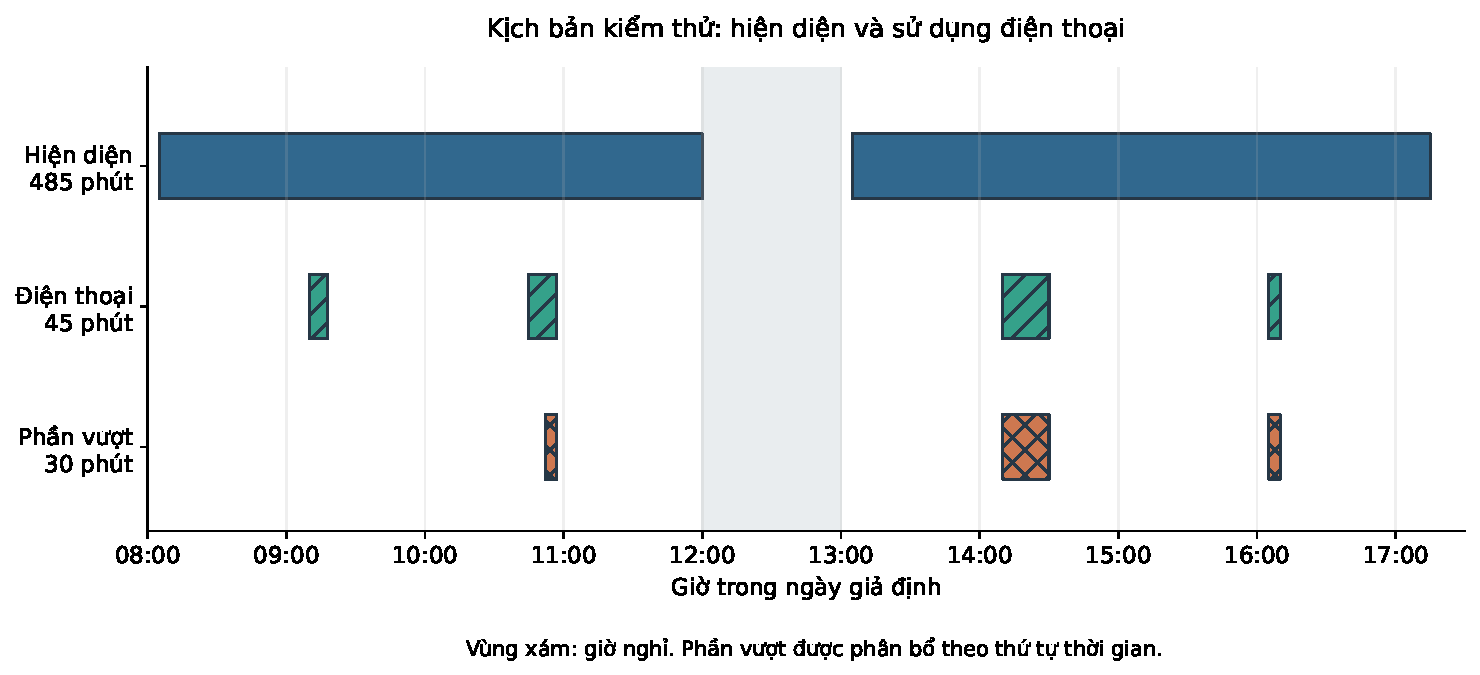
\includegraphics[width=0.93\textwidth]{Images/sim_timeline.pdf}
\caption{Dòng thời gian tổng hợp về hiện diện, điện thoại và phần vượt hạn mức}
\label{fig:timeline-ui}
\end{figure}

Hình được tạo từ các khoảng thời gian công bố tại mục~\ref{sec:policy-sensitivity}. Tổng hiện diện là 485 phút, điện thoại 45 phút và hạn mức 15 phút, cho thời gian hiệu lực 455 phút. Hàng cuối thể hiện phần điện thoại vượt hạn mức theo thứ tự thời gian, không biểu diễn năng suất từng đoạn.

\subsubsection{Trang chi tiết nhân viên}
Dòng thời gian sự kiện có bộ lọc hiện diện/điện thoại/danh tính/gián đoạn camera. Mỗi khoảng thời gian hiển thị mốc bắt đầu, mốc kết thúc, thời lượng, nguồn sự kiện và độ tin cậy. Nếu có bằng chứng, chỉ người dùng có quyền mới thấy nút mở ảnh. Hậu kiểm được lưu riêng không ghi đè sự kiện.

\subsection{Lưu trữ bằng chứng và báo cáo}
Ảnh chụp không lưu liên tục. Mặc định có thể lưu khi danh tính không khớp, khi tổng thời gian điện thoại lần đầu vượt hạn mức hoặc khi người giám sát yêu cầu chụp thủ công. Đường dẫn tệp do máy chủ sinh từ tổ chức/phiên/mã sự kiện, kiểm tra traversal và mã băm để phát hiện hỏng tệp.

Tiến trình nền sinh báo cáo nhận \texttt{ReportJob}, tải bản tổng hợp/khoảng thời gian/sự kiện, kết xuất Jinja2 sang HTML rồi chuyển PDF. Báo cáo cá nhân gồm bảng tổng thời gian, dòng thời gian, danh sách phiên sử dụng điện thoại và thời gian camera không quan sát được. Báo cáo tổ chức tổng hợp nhiều nhân viên nhưng không mặc định nhúng ảnh.

\subsection{Ghi nhật ký và khả năng quan sát}
Ứng dụng phía máy khách ghi thời gian xử lý từng công đoạn, số quan sát phát hiện, số quỹ đạo đang hoạt động, số lần nghi ngờ đổi định danh theo quy tắc chẩn đoán, độ dài hàng đợi và FPS của camera. Máy chủ ứng dụng ghi mã yêu cầu, mã sự kiện, mã phiên camera, tác vụ báo cáo. Không ghi token hoặc vector đặc trưng khuôn mặt vào nhật ký. Chỉ số hữu ích gồm \texttt{camera\_last\_seen}, \texttt{pipeline\_latency}, \texttt{ws\_queue\_lag}, số sự kiện gửi lại và số khung hình UNKNOWN.

\subsection{Kiểm thử mã nguồn}
\subsubsection{Kiểm thử đơn vị}
Kế hoạch kiểm thử đơn vị bao phủ IoU/hình học, point-in-polygon, điểm neo, các phép chuyển trạng thái, truy hồi mốc thời gian, phép giao khoảng thời gian, hạn mức/phần vượt hạn mức, liên kết người sử dụng điện thoại, biên chênh lệch khi xác minh danh tính và khả năng xử lý sự kiện lặp mà không nhân đôi kết quả.

\subsubsection{Kiểm thử tích hợp}
Kiểm thử tích hợp dự kiến dùng video ngắn để chạy từ bộ phát hiện đến máy chủ. Khi dùng kết quả phát hiện giả định, phép thử bắt đầu sau bộ phát hiện và không đánh giá chất lượng nhận biết. TestClient được dùng ở ranh giới API. Kịch bản gồm người vào/ra, che khuất 3 giây, mất 8 giây, hai người đổi vị trí, điện thoại của người A gần người B, camera mất kết nối và kết nối lại.

\subsubsection{Kiểm thử bảo mật}
Kế hoạch kiểm thử máy chủ gồm cô lập dữ liệu giữa các tổ chức, vai trò, mã xác thực camera, quyền truy cập bằng chứng, path traversal, WebSocket ticket/phát lại, rate limit và chính sách CORS và HTTPS. Các kiểm thử này kế thừa tư tưởng từ mã nguồn nền nhưng đổi tài nguyên theo miền mới.

\subsection{Triển khai}
Máy chủ ứng dụng Compose gồm ứng dụng, PostgreSQL, Redis và volume bằng chứng/báo cáo. SQLite có thể phục vụ một số kiểm thử cục bộ, nhưng các ràng buộc và giao dịch cần được kiểm thử lại trên PostgreSQL trước khi triển khai. Ứng dụng camera được cấu hình URL máy chủ và token riêng. Nếu GPU tại thiết bị biên không có, có thể giảm kích thước đầu vào suy luận/FPS hoặc dùng mô hình nano, các lựa chọn phải được ghi trong siêu dữ liệu kết quả đánh giá.

\begin{table}[H]
\centering
\caption{Thành phần triển khai}
\label{tab:deployment}
\begin{tabularx}{\textwidth}{p{3.2cm}p{4cm}X}
\toprule
\textbf{Nút triển khai} & \textbf{Thành phần} & \textbf{Dữ liệu chính}\\
\midrule
Thiết bị biên camera & ứng dụng thị giác tại thiết bị biên, mô hình, hàng đợi cục bộ & Khung hình tạm, quỹ đạo/trạng thái, sự kiện chờ ACK\\
Máy chủ ứng dụng & FastAPI, tiến trình xử lý nền & API, WebSocket, báo cáo\\
PostgreSQL & Quan hệ/trạng thái hiện tại & User, nhân viên, camera, các khoảng thời gian, bản tổng hợp\\
Redis & Cache/phân phối cập nhật/tác vụ & Dữ liệu tạm thời\\
Vùng lưu trữ bằng chứng & Ảnh chụp/báo cáo & Tệp có thời hạn lưu trữ\\
Trình duyệt & Bảng điều khiển & Dữ liệu đã phân quyền\\
\bottomrule
\end{tabularx}
\end{table}

\subsection{Các lỗi biên cần xử lý}
Các trường hợp đặc biệt gồm: người ngồi thấp khiến điểm giữa cạnh đáy hộp bao nằm ngoài ROI, hai người đứng chung vùng, điện thoại cầm gần ranh giới hai người, mã quỹ đạo khởi tạo lại khi camera kết nối lại, khuôn mặt nhỏ không đủ vector đặc trưng, mốc thời gian camera thay đổi đột ngột, lịch làm việc thay đổi sau khi bản tổng hợp đã sinh. Mỗi trường hợp cần chính sách rõ: UNKNOWN thay vì đoán, phiên bản cấu hình, khóa bản tổng hợp theo phiên bản chính sách và cho phép tính lại có kiểm toán.

\subsection{Cài đặt vòng lặp xử lý camera}
Vòng lặp camera được tách thành thu nhận, suy luận và truyền dữ liệu. Luồng thu nhận chỉ đọc nguồn, đóng gói \texttt{FramePacket} và đưa vào hàng đợi giới hạn. Tiến trình suy luận lấy khung hình mới nhất phù hợp với chính sách lấy mẫu, chạy bộ phát hiện/bộ theo dõi/ngữ cảnh rồi cập nhật trạng thái. Tiến trình truyền dữ liệu gửi sự kiện và telemetry, lỗi mạng không được chặn suy luận.

Một hàng đợi khung hình dài gây ra hiện tượng hệ thống xử lý quá khứ. Vì mục tiêu là giám sát gần thời gian thực, hàng đợi dùng chính sách drop-oldest khi đầy. Mỗi gói khung hình có \texttt{captured\_at} và \texttt{enqueued\_at}, tiến trình xử lý nền đo tuổi khung hình trước suy luận. Nếu tuổi khung hình vượt ngưỡng, khung hình bị bỏ và chỉ số tăng. Ngược lại, hàng đợi sự kiện không dùng drop-oldest vì sự kiện là dữ liệu nghiệp vụ.

Trình tự xử lý một khung hình được mô tả bằng mã giả sau:
\begin{Verbatim}[fontsize=\small,breaklines=true]
packet = frame_queue.get_latest()
if packet.age_ms > config.max_frame_age_ms:
    metrics.increment("stale_frame")
    continue

result = detector.infer(packet)
tracks = tracker.update(result.person_detections, packet.source_time)
contexts = roi_manager.assign(tracks, active_work_areas)
identities = identity_scheduler.update(packet, tracks, contexts)
phone_links = phone_associator.assign(
    result.phone_detections, tracks, contexts
)

observations = build_observations(
    contexts, identities, phone_links,
    active_state_keys=state_registry.active_keys(),
)
for observation in observations:
    transitions = state_registry.update(observation, packet.source_time)
    event_queue.append_all(transitions)
\end{Verbatim}

Mỗi bước nhận dữ liệu bất biến của khung hình hiện tại. Mọi hộp bao được chuyển về khung hình gốc ngay sau bộ phát hiện để ROI và bằng chứng dùng cùng hệ tọa độ. Hàm tạo quan sát phải cập nhật cả trạng thái đang mở nhưng không còn quỹ đạo xuất hiện, với NOT\_DETECTED khi khung hình hợp lệ và UNKNOWN khi nguồn không hợp lệ. Nếu chỉ duyệt các quỹ đạo vừa phát hiện, trạng thái cũ có thể không bao giờ nhận tín hiệu để kết thúc. Khi nguồn ngừng trả khung hình, bộ giám sát nguồn vẫn phải kích hoạt xử lý gián đoạn theo thời gian chờ.

\subsection{Quản lý cấu hình và phiên bản}
Cấu hình được chia thành bốn nhóm: mô hình, camera, xử lý thời gian và chính sách. Mô hình chứa mã kiểm tra trọng số, kích thước đầu vào suy luận, mã lớp và độ tin cậy. Camera chứa nguồn, độ phân giải kỳ vọng, ROI và calibration. Nhóm thời gian chứa $T_{enter}$, $T_{gap}$, $T_{phone\_enter}$, $T_{phone\_exit}$ và bộ đệm của bộ theo dõi. Chính sách chứa lịch làm việc, hạn mức, quy tắc danh tính và thời hạn lưu trữ.

Ứng dụng phía máy khách kiểm tra lược đồ khi khởi động. Giá trị thời gian phải không âm, ngưỡng độ tin cậy nằm trong $[0,1]$, đa giác hợp lệ, ngưỡng reject nhỏ hơn ngưỡng accept. Cấu hình sai làm ứng dụng chuyển sang CONFIGURATION\_ERROR. Bộ tính tham chiếu cũng từ chối hạn mức âm, số không hữu hạn, cờ điều chỉnh sai kiểu và khoảng có mốc kết thúc trước mốc bắt đầu.

Khi máy chủ phát cấu hình mới, ứng dụng phía máy khách tải về vùng lưu trữ tạm, kiểm tra chữ ký/mã kiểm tra và xác thực. Các thay đổi không ảnh hưởng hình học có thể áp dụng tại ranh giới khung hình, thay đổi ROI, mô hình hoặc bộ theo dõi cần ranh giới phiên để tránh một khoảng thời gian dùng hai ngữ nghĩa. Sự kiện CONFIG\_ACTIVATED ghi phiên bản và thời điểm bắt đầu hiệu lực.

\subsection{Cài đặt kho trạng thái theo phiên camera}
\texttt{StateRegistry} ánh xạ khóa $(session\_id, track\_id)$ tới ngữ cảnh và các FSM. Kho trạng thái chịu trách nhiệm khởi tạo trạng thái khi quỹ đạo mới, cập nhật khi quỹ đạo hoạt động và thu hồi trạng thái sau khi quỹ đạo kết thúc đủ lâu. Thu hồi phải gọi hàm finalize để đóng phiên còn mở trước khi giải phóng bộ nhớ.

Không dùng mã quỹ đạo đơn lẻ làm khóa toàn cục. Khi bộ theo dõi khởi tạo lại, ID có thể bắt đầu lại từ 1. Ghép cùng mã phiên bảo đảm hai quỹ đạo khác phiên không chia sẻ trạng thái. Mã nhân viên chỉ được gắn sau liên kết, nếu danh tính thay đổi từ PROVISIONAL sang VERIFIED, khoảng thời gian hiện tại cập nhật siêu dữ liệu chứ không đổi khóa FSM.

Checkpoint kho trạng thái được ghi định kỳ bằng thao tác nguyên tử: ghi tệp tạm, đồng bộ dữ liệu xuống thiết bị lưu trữ rồi đổi tên. Checkpoint không chứa khung hình hoặc vector đặc trưng, chỉ có trạng thái cần phục hồi. Nếu checkpoint hỏng mã kiểm tra, ứng dụng phía máy khách bỏ checkpoint, tạo phiên mới và phát RECOVERY\_FAILED để máy chủ đánh dấu khoảng không chắc chắn.

\subsection{Cài đặt bộ lập lịch xác minh danh tính}
Chạy FaceNet cho mọi quỹ đạo ở mọi khung hình vừa tốn tài nguyên vừa tạo nhiều phép so sánh trên ảnh cắt chất lượng thấp. \texttt{IdentityScheduler} chỉ tạo tác vụ khi quỹ đạo đủ tuổi, nằm trong ROI, mặt đạt kích thước/chất lượng tối thiểu và không có kết quả VERIFIED còn hiệu lực.

Chất lượng cắt vùng ảnh có thể kết hợp kích thước mặt, độ mờ và góc nhìn. Phương sai của đáp ứng Laplace có thể được dùng như tín hiệu độ nét nhưng không phải tiêu chí duy nhất. Tác vụ được đưa vào hàng đợi ưu tiên, quỹ đạo chưa từng xác minh có ưu tiên cao hơn quỹ đạo đã VERIFIED gần đây. Mỗi quỹ đạo có thời gian chờ tối thiểu giữa hai lần xác minh để tránh tạo nhiều tác vụ khi tiến trình xử lý nền chậm.

Vector đặc trưng tham chiếu của một nhân viên có thể gồm nhiều mẫu. Thay vì chỉ lấy một vector trung bình trong mọi trường hợp, hệ thống lưu vector trung tâm và thống kê phân tán, điểm liên kết ứng viên có thể lấy khoảng cách nhỏ nhất có kiểm soát hoặc khoảng cách tới vector trung tâm. Phiên bản mô hình phải khớp vì vector đặc trưng từ hai mô hình khác nhau không được so sánh trực tiếp.

\subsection{Cài đặt thuật toán PhoneAssociator}
Với mỗi hộp bao điện thoại, bộ liên kết xây dựng tập người ứng viên dựa trên vùng tương tác và vùng ngữ cảnh. Điểm liên kết sử dụng tỉ lệ hộp điện thoại nằm trong vùng thân trên, khoảng cách tâm chuẩn hóa và tính nhất quán với ROI:
\begin{equation}
 S(p,q)=w_1\frac{|p\cap U(q)|}{|p|}+w_2(1-d_n(p,q))+w_3R(p,q).
\end{equation}
Trong công thức, $p$ là hộp điện thoại có diện tích dương, $U(q)$ là vùng tương tác của người và $w_i\geq0$, $\sum_iw_i=1$. Tỉ lệ bao chứa dùng diện tích điện thoại làm mẫu số để tránh điểm IoU rất nhỏ chỉ do chênh lệch kích thước giữa điện thoại và người. Các trọng số và ngưỡng được lưu trong cấu hình. $d_n$ được chuẩn hóa theo chiều cao hộp bao người và giới hạn trong $[0,1]$ để một khoảng cách pixel có ý nghĩa tương đối nhất quán ở gần và xa camera.

Liên kết thực hiện theo từng điện thoại và giải quyết xung đột toàn cục. Nếu hai điện thoại cùng chọn một người, chính sách có thể giữ hộp bao có độ tin cậy cao nhất hoặc cho phép nhiều vật thể nhưng chỉ một trạng thái hành vi sử dụng điện thoại. Nếu một điện thoại có hai người gần bằng nhau, trả UNKNOWN. Kết quả ghi cả điểm liên kết cao nhất, điểm liên kết cao thứ hai và biên chênh lệch để phân tích lỗi.

\begin{Verbatim}[fontsize=\small,breaklines=true]
candidates = score_candidates(phone_box, active_tracks)
if not candidates:
    return UNASSIGNED
best, second = top_two(candidates)
if best.score < min_score:
    return UNASSIGNED
if second and best.score - second.score < min_margin:
    return AMBIGUOUS
return ASSIGNED(best.track_id, best.score)
\end{Verbatim}

\subsection{Cài đặt bộ tổng hợp khoảng thời gian}
Bộ tổng hợp không cộng thời lượng từ các dòng chưa chuẩn hóa. Hàm \texttt{normalize\_intervals} sắp xếp, cắt theo miền hợp lệ và hợp nhất khoảng chồng lấn. Sau đó \texttt{intersect\_sets} tính giao hiện diện với lịch làm việc và điện thoại với hiện diện hợp lệ.

Các phép tính thời lượng sử dụng số nguyên mili giây hoặc số thập phân có độ chính xác kiểm soát, tránh tích lũy sai số từ phép cộng số thực dấu phẩy động theo từng khung hình. Khi hiển thị, giá trị được làm tròn ở lớp hiển thị, cơ sở dữ liệu giữ độ chính xác gốc. Quy tắc làm tròn cần thống nhất, ví dụ tổng theo mili giây rồi làm tròn một lần, tránh làm tròn từng phiên gây sai số cộng dồn.

\begin{Verbatim}[fontsize=\small,breaklines=true]
observed_schedule = subtract_sets(
    normalize_intervals(schedule_intervals),
    normalize_intervals(unobserved_intervals),
)
valid_presence = intersect_sets(
    normalize_intervals(presence_intervals),
    observed_schedule,
)
valid_phone = intersect_sets(
    normalize_intervals(phone_intervals),
    valid_presence,
)
gross_ms = duration(valid_presence)
phone_ms = duration(valid_phone)
excess_ms = max(0, phone_ms - allowance_ms)
effective_ms = max(0, gross_ms - excess_ms) if deduction_enabled else gross_ms
\end{Verbatim}

Nếu có gián đoạn quan sát, bộ tổng hợp tính $\texttt{unobserved\_ms}=|\textit{schedule}\cap\textit{outage}|$. Độ bao phủ bằng phần lịch làm việc được quan sát chia tổng lịch làm việc. Bản tổng hợp độ bao phủ thấp được đánh cờ, trong phạm vi thiết kế này, hệ thống không nội suy hiện diện qua khoảng mất camera.

\subsection{Cài đặt API xử lý lặp an toàn}
Điểm cuối API nhận sự kiện yêu cầu \texttt{event\_id} và mã xác thực camera. Giao dịch kiểm tra token, chèn sự kiện với khóa duy nhất, cập nhật cursor và tạo bản ghi hộp thư sự kiện. Nếu mã sự kiện đã tồn tại với cùng mã băm nội dung thông điệp, máy chủ trả kết quả cũ. Nếu cùng ID nhưng nội dung thông điệp khác, máy chủ trả lỗi xung đột và ghi nhật ký bảo mật.

Mẫu thiết kế hộp thư sự kiện (outbox) giúp việc lưu cơ sở dữ liệu và phát thông báo không bị lệch. Sự kiện và outbox được xác nhận trong một giao dịch. Tiến trình xử lý nền đọc outbox, cập nhật trạng thái dẫn xuất đã lưu và phân phối cập nhật, nếu tiến trình xử lý nền dừng đột ngột, bản ghi chưa đánh dấu hoàn tất sẽ được xử lý lại một cách idempotent.

REST API danh sách dùng phân trang bằng con trỏ ổn định theo $(occurred\_at,id)$ thay vì offset lớn. Các điểm cuối API tải bằng chứng không nhận đường dẫn tệp, chúng nhận mã bằng chứng, kiểm tra tổ chức/quyền truy cập rồi tạo phản hồi hoặc URL có chữ ký ngắn hạn.

\subsection{Cài đặt WebSocket và kiểm soát áp lực ngược khi bên nhận quá tải}
Khi kết nối, bảng điều khiển dùng phiên xác thực để nhận vé kết nối dùng một lần. Máy chủ WebSocket xác thực ticket, tạo đăng ký nhận dữ liệu theo tổ chức/camera được phép và gửi \texttt{hello} chứa thời gian máy chủ/phiên bản lược đồ. Ứng dụng phía máy khách tải bản chụp trạng thái qua REST trước hoặc ngay sau hello rồi áp dụng phần cập nhật có số thứ tự lớn hơn con trỏ của bản chụp trạng thái.

Mỗi kết nối có hàng đợi giới hạn. Nếu trình duyệt xử lý chậm, máy chủ hợp nhất các cập nhật trạng thái hiện tại cùng khóa và giữ sự kiện quan trọng. Khi hàng đợi vẫn vượt ngưỡng, máy chủ đóng kết nối với mã rõ ràng, ứng dụng phía máy khách kết nối lại và tải bản chụp trạng thái mới. Cách này tránh một bên nhận dữ liệu chậm làm tăng bộ nhớ toàn máy chủ.

Thông điệp có \texttt{message\_type}, \texttt{schema\_version}, \texttt{cursor} và \texttt{payload}. Trình duyệt bỏ qua loại thông điệp chưa biết nhưng không được bỏ qua thay đổi phiên bản chính của lược đồ. Ping/pong đo kết nối, không thay thế tín hiệu duy trì kết nối nghiệp vụ của camera.

\subsection{Chuyển đổi lược đồ và tính tương thích dữ liệu}
Lược đồ cơ sở dữ liệu thay đổi qua chuyển đổi lược đồ có phiên bản. Thay đổi phá vỡ được triển khai theo expand--migrate--contract: thêm cột/bảng mới tương thích, bổ sung dữ liệu lịch sử theo lô, chuyển ứng dụng sang đọc mới, sau đó mới loại trường cũ. Không đổi tên/xóa cột trong cùng lần triển khai mà ứng dụng phía máy khách cũ còn sử dụng.

Bổ sung dữ liệu lịch sử bản tổng hợp cần lưu tiến độ và chạy idempotent. Với bảng lớn, tác vụ xử lý theo khoảng ID hoặc ngày để tránh giao dịch dài. Sau chuyển đổi lược đồ, kiểm tra số dòng, ràng buộc, bản ghi mẫu và khả năng khôi phục phiên bản ứng dụng trước đó. Việc khôi phục lược đồ chỉ thực hiện khi bảo đảm không mất dữ liệu.

\subsection{Xử lý lỗi và chiến lược phục hồi}
Lỗi được phân loại thành tạm thời, cấu hình, dữ liệu và không thể phục hồi. Lỗi mạng hoặc thời gian chờ là tạm thời và gửi lại có thời gian chờ tăng dần. Đa giác sai hoặc mô hình thiếu là lỗi cấu hình, cần can thiệp thay vì gửi lại vô hạn. Sự kiện trái lược đồ là lỗi dữ liệu và đưa vào hàng đợi lỗi. Lỗi bộ nhớ hoặc hỏng dữ liệu có thể yêu cầu dừng phiên.

Mỗi lỗi có mã ổn định, thông báo người vận hành và ngữ cảnh không nhạy cảm. Không bắt ngoại lệ chung rồi tiếp tục trong máy trạng thái vì có thể làm trạng thái âm thầm sai. Tại ranh giới vòng lặp, lỗi một khung hình có thể được ghi và bỏ khung hình, lỗi bất biến trạng thái phải dừng phiên hoặc khởi tạo lại có kiểm soát.

\begin{table}[H]
\centering
\caption{Chính sách xử lý lỗi theo nhóm}
\label{tab:error-handling-implementation}
\begin{tabularx}{\textwidth}{p{3cm}p{3.3cm}X X}
\toprule
\textbf{Nhóm} & \textbf{Ví dụ} & \textbf{Phản ứng} & \textbf{Quan sát}\\
\midrule
Lỗi tạm thời & hết thời gian chờ RTSP, HTTP 503 & Gửi lại với thời gian chờ tăng dần, giữ hàng đợi & Số lần gửi lại, thời gian gián đoạn\\
Cấu hình & ROI sai, thiếu bộ trọng số & Dừng kiểm tra trước khi chạy & Mã lỗi, phiên bản cấu hình\\
Dữ liệu & Sự kiện sai lược đồ & Từ chối và lưu hàng đợi lỗi & Mã băm nội dung thông điệp, phiên bản bên gửi\\
Tài nguyên & Ổ đĩa hoặc hàng đợi gần đầy & Giảm telemetry, cảnh báo & Mức sử dụng tài nguyên, thời gian lưu trong hàng đợi\\
Vi phạm bất biến nghiêm trọng & Khoảng thời gian âm, trạng thái hỏng & Dừng phiên an toàn & Báo cáo sự cố, checkpoint\\
\bottomrule
\end{tabularx}
\end{table}

\subsection{Tổ chức kiểm thử theo lớp}
Bộ phát hiện, đồng hồ, nguồn khung hình và kênh truyền sự kiện đều có giao diện trừu tượng để thay bằng đối tượng thay thế khi kiểm thử. Bộ phát hiện giả lập phát hộp bao theo kịch bản định trước, đồng hồ giả lập cho phép tiến thời gian mà không cần chờ theo thời gian thực, kênh truyền giả lập mô phỏng mất ACK, gửi trùng và đảo thứ tự. Nhờ đó máy trạng thái được kiểm thử theo cách xác định.

Kiểm thử dựa trên thuộc tính phù hợp với khoảng thời gian: kết quả chuẩn hóa không chồng lấn, thời lượng không âm, giao không dài hơn mỗi tập đầu vào, hiệu lực không lớn hơn tổng hiện diện và không âm. Máy trạng thái có thể sinh chuỗi quan sát ngẫu nhiên và kiểm tra bất biến tối đa một khoảng thời gian mở.

Kiểm thử đối chiếu kết quả chuẩn dùng một tệp quan sát phát hiện/quỹ đạo đã ghi để so sự kiện và bản tổng hợp mong đợi. Khi thuật toán thay đổi có chủ ý, người rà soát xem khác biệt tệp kết quả trước khi cập nhật kết quả chuẩn. Điều này phát hiện thay đổi ngữ nghĩa ngoài dự kiến tốt hơn chỉ kiểm tra chương trình không dừng đột ngột.

\subsection{Quy trình phát hành và vận hành}
Chuỗi xử lý tích hợp liên tục (CI) thực hiện định dạng và kiểm tra tĩnh, kiểm thử đơn vị, kiểm thử tích hợp, kiểm tra chuyển đổi lược đồ, đóng gói ảnh triển khai và quét thư viện phụ thuộc. Ảnh triển khai được gắn commit SHA, trọng số mô hình có mã kiểm tra riêng. Môi trường thử nghiệm chạy video kịch bản trước khi phát hành sang môi trường vận hành.

Triển khai máy chủ theo cập nhật lần lượt nếu lược đồ tương thích. Ứng dụng camera có thể triển khai thăm dò trên một số thiết bị, chỉ số UNKNOWN, độ trễ và lỗi sự kiện được so với phiên bản trước. Nếu xấu đi, khôi phục phiên bản trước ứng dụng phía máy khách nhưng giữ sự kiện đã sinh, lược đồ có phiên bản bảo đảm máy chủ hiểu cả hai ứng dụng phía máy khách trong cửa sổ chuyển đổi.

Sao lưu gồm PostgreSQL và siêu dữ liệu bằng chứng, tệp bằng chứng cần chiến lược riêng theo thời hạn lưu trữ. Kiểm thử phục hồi phải được thực hiện định kỳ, vì bản sao lưu tồn tại nhưng không phục hồi được không có giá trị. Tài liệu hướng dẫn vận hành ghi rõ RPO/RTO mục tiêu, người chịu trách nhiệm và cách xác minh sau phục hồi.

\subsection{Kết luận chương}
Phương án cài đặt tách suy luận thị giác khỏi quy tắc tổng hợp theo chính sách. Bộ phát hiện/bộ theo dõi tạo quan sát, ngữ cảnh/trạng thái chuyển quan sát thành khoảng thời gian, bộ tổng hợp áp dụng lịch làm việc/chính sách, máy chủ ứng dụng lưu, phân quyền và trình bày. Sự phân tách này cho phép thay YOLO hoặc bộ theo dõi mà không phải viết lại cách tính thời gian và cho phép kiểm thử riêng bộ tính thời gian trước khi tích hợp chuỗi xử lý video. Chương 6 trình bày kết quả đã thực thi cho bộ tính này và kế hoạch kiểm chứng các thành phần còn lại.
